\documentclass[a4paper,12pt,titlepage]{report}

\usepackage[toc,page]{appendix}
\usepackage[hidelinks]{hyperref}
\usepackage{fullpage}
\usepackage{caption}
\usepackage{pgfgantt}
\usepackage{subcaption}
\usepackage{minted}
\usepackage{todonotes}
\usepackage[backend=bibtex]{biblatex}
\usepackage[acronym,nomain]{glossaries}
\usepackage[tablegrid]{vhistory}
\usepackage{tikz}
\usetikzlibrary{shapes, positioning}

\RecustomVerbatimEnvironment{Verbatim}{BVerbatim}{}
\renewcommand{\figurename}{Listing}

\bibliography{report}
\makeglossaries

% Number subsubsections
\setcounter{secnumdepth}{3}

\begin{document}

  \newacronym{gc}{G.C.}{Garbage Collector}
\newacronym{dos}{DoS}{Denial of Service}
\newacronym{fifo}{FIFO}{First-In-First-Out}
\newacronym{iot}{IoT}{Internet of Things}
\newacronym{sla}{SLA}{Service Level Agreement}
\newacronym[longplural={Remote Procedure Calls}]{rpc}{RPC}{Remote Procedure Call}
\newacronym{rtt}{RTT}{Round-trip time}
\newacronym{soa}{SoA}{Service Oriented Architecture}
\newacronym{json}{JSON}{JavaScript Object Notation}
\newacronym{tcp}{TCP}{Transmission Control Protocol}


  \begin{titlepage}
    \begin{center}
        \vspace*{1cm}

        \Huge
        \textbf{Writing a Message Broker in GoLang}

        \vspace{2.0cm}
        \LARGE

        \textbf{George Vanburgh}

        \vspace{0.5cm}
        Supervised by Alvaro A.A. Fernandes

        \vspace{0.5cm}
        Draft \today

        \vfill

        
\includegraphics[width=0.4\textwidth]{figures/manchester}

        \vspace{0.8cm}
        \large

        A report submitted in part fulfilment of the degree of \\
        \textbf{BSc (Hons) in Computer Science with Industrial Experience}

    \end{center}
  \end{titlepage}

  \begin{abstract}
    An exercise in building a feature-rich application message broker using Google's
new 'GoLang' programming language, modern software engineering techniques and
best practises. Evaluation of my produced broker is achieved through both
black-and-white-box testing, as well as comparisons to existing commercial
solutions.

  \end{abstract}

  \renewcommand{\abstractname}{Acknowledgements}
  \begin{abstract}
  \end{abstract}

  \tableofcontents
  \begin{versionhistory}
    \vhEntry{0.1}{05.10.15}{GV}{Creation}
    \vhEntry{0.2}{12.10.15}{GV}{Initial background section}
    \vhEntry{0.3}{06.02.16}{GV}{Basic report structure}
    \vhEntry{0.4}{30.03.16}{GV}{New title page, and stubbed out sections}
  \end{versionhistory}
  \newpage

  \section{Introduction}
\label{sec:Introduction}

\subsection{Background}
\label{sub:Background}

Many large, distributed applications (particularly in 'enterprise' environments)
make extensive use of messaging brokers -
software (or hardware in some cases\cite{solaceappliances}) responsible for passing
layer-7 messages between services, over the network. Two examples of message
brokers are
\href{http://www.tibco.com/products/automation/enterprise-messaging/enterprise-message-service}{TibcoEMS}
and \href{https://www.rabbitmq.com/}{RabbitMQ}.

\subsection{Overview}
\label{sub:Overview}

This project centers around building an enterprise-style messaging broker,
as an exercise in understanding the various challenges associated with middleware
communications under various networking conditions. These conditions are
representative of the various different environments an application is expected
to operate in. For example, an Internet of Things device that wishes to send information back
to a cloud-based data collector - has a fundamentally different set of priorities
to a server exchanging messages within a local datacenter, say as part of a large
financial application. For example - an \gls{iot} device may
have constrains placed on its battery life - meaning that reducing the amount of
energy consumed in sending each message would take precedence over the
requirement to, say, deliver messages in order. The project will center around
designing and implementing various 'strategies' for meeting the kinds of SLA
found in these discreet environment - and evaluating the performance of each
strategy under various different workloads and scenarios.


  \section{Background}
\label{sec:Background}


  \chapter{Design}
\label{chap:Design}

\section{Project philosophy}
\label{sec:Project philosophy}

One of the learning objectives for this project, was to discover and utilize
\gls{foss} technologies wherever possible, as well as give back to the
\gls{foss} community. As such, all of the tooling used in the production of the
project, as well as the project itself were open-source. The project itself is
published under the MIT License, which allows anyone to "use, copy, modify,
merge, publish, distribute, sublicense, and/or sell copies of the Software",
without restriction.

\section{Presentation interface}
\label{sec:presentation}

As a (primarily) middleware project - coming up with a compelling presentation
interface is crucial to allowing people to engage with the software, as well as
providing monitoring capabilities, should it be deployed in a production
environment. Broker metrics such as:

\begin{itemize}
  \item Messages/second (broken down by topic)
  \item (Average) End-to-end latency for each message
  \item Memory/Disk usage
  \item CPU utilisation
  \item Pending messages
  \item Unacknowledged messages
  \item Total messages processed
\end{itemize}

And client metrics such as:

\begin{itemize}
  \item Messages sent
  \item Messages received
  \item Messages lost
\end{itemize}

Should be easily accessible, and visualised. The presentation and metrics
collection for gamq consists of the following components:

\subsection{StatsD}
\label{sub:StatsD}

StatsD is an open-source statistics daemon, written by developers at
Etsy\footnote{\url{https://www.etsy.com/uk/}} in 2010\cite{statsd}, and which
has seen widespread adoption by infrastructure teams ever since. StatsD aims to
define a simple protocol (Listing~\ref{lst:statsdSchema}) for sending statistics
over the network, and make it simple to aggregate and store those metrics for
real-time analysis. StatsD can differentiate between metrics of different types:

\begin{listing}
  \centering
  \mintinline{text}{metricname:1|c}
  \caption{A simple counter metric, exactly as it would appear inside a network packet}
  \label{lst:statsdSchema}
\end{listing}

\begin{description}
  \item[Counters] A simple counter that can be incremented or decremented. An
  example use case could be the number of messages sent through a broker.
  \item[Timing] The amount of time taken to complete a task. An example could be
  the amount of time taken to process a message.
  \item[Gauges] An arbitrary value, stored until it is superseded by a new
  value. An example of this could be the number of connections open to the
  broker at a single point in time.
\end{description}

These packets can be sent over the network as either TCP or UDP packets. Packets
can contain multiple metrics, separated with newline characters
(Listing~\ref{lst:statsdMultiplePackets}), which can greatly improve the
efficiency of the transfer, as the size of each metric (the order of a few
bytes) is far below the maximum capacity of a single packet.\footnote{The
typical \gls{mtu} of Ethernet networks is ~1500 bytes} Gamq uses the UDP
protocol by default (although this is configurable, see
Section~\ref{sec:Configuration} for details), as the cost of sending UDP packets
is very low cost when compared to TCP, and we do not require the deliverability
guarantees of TCP (metrics are non-critical). Metrics are typically sent over a
\gls{lan}, where packet loss is usually quite low. In the event that is it not,
but the packet loss is uniform, the loss of some metrics should not affect the
overall data trend.

\begin{listing}
  \centering
  \mintinline{text}{gorets:1|c\nglork:320|ms\ngaugor:333|g\nuniques:765|s}
  \caption{Multiple metrics in a single packet}
  \label{lst:statsdMultiplePackets}
\end{listing}

\subsection{InfluxDB}
\label{sub:InfluxDB}

InfluxDB is an open-source, NoSQL database, optimised for the storage and
retrieval of \gls{time-series data}. Influx is part of a family of databases
designed to store (amongst other things) a large amount of metrics data at very
high speed (the order of millions of events per second), which also includes
\href{http://graphite.wikidot.com/}{Graphite} and
\href{http://opentsdb.net/}{OpenTSDB}. InfluxDB was chosen for this project due
to its maturity (compared to OpenTSDB) and performance (compared to
Graphite/Carbon).

\subsection{Grafana}
\label{sub:Grafana}

\href{http://grafana.org/}{Grafana} is an open-source visualisation tool for
\gls{time-series data}, typically that which is produced by Internet
infrastructure and application analytics. Developed by a consortium of Internet
companies as a modern replacement for the previously popular
\href{https://github.com/graphite-project/graphite-web}{Graphite-Web} project.
Grafana can visualise \gls{time-series data} from a variety of data-sources,
such as the ElasticSearch, the aforementioned Graphite and, most importantly,
InfluxDB.

\missingfigure{Grafana screenshot}

\subsection{Docker}
\label{sub:dockerDesign}

Gamq is designed to send StatsD messages (Section~\ref{sub:StatsD}) across the
network. In a production environment, these would be sent to the above software
stack, running on a separate server in the datacenter. In a development
environment, the metrics stack could be run on a development server, or the
developers local machine. The configured stack should therefore be as portable
as possible, to make development as simple as possible. \todo{Docker description}

\section{Configuration}
\label{sec:Configuration}

As with most pieces of software - there are situations where the default
behaviour of a message broker requires adjustment to suit its operating
environment. One example of this is the network port that the broker operates
on, and which other applications will connect to in order to exchange messages.
Whilst the default port (48879\footnote{A number chosen due to its memorable
hexadecimal representation: \texttt{0xBEEF}} in the case of this broker) may be
suitable in most cases, since no other 'well-known' applications use that
particular
port.\footnote{\url{https://en.wikipedia.org/wiki/List_of_TCP_and_UDP_port_numbers}}.

\subsection{Command-line configuration}
\label{sub:Command-line configuration}

A number of these configurable parameters make sense to expose as command-line
parameters, specified at application start time. The available parameters can be
exposed using the \texttt{--help} parameter, the output of which can be seen in
Listing~\ref{lst:gamqHelpOutput}

\begin{listing}[ht]
  \centering
  \inputminted{bash}{code/gamqHelpOutput}
  \caption{Output of running the broker with the --help flag}
  \label{lst:gamqHelpOutput}
\end{listing}

\subsection{File-based configuration}
\label{sub:File-based configuration}

Whilst specifying arguments on the command line gives flexibility, there are
certain options that, whilst configurable, are either too numerous, or change
too infrequently to justify command-line flags. One major example of this is the
log configuration for the broker - an \gls{xml} file specifying specifying the
format, and location of messages logged using the
\href{https://github.com/cihub/seelog}{Seelog} library. An example log
configuration can be seen in Listing~\ref{lst:seelogConfig}.

\begin{listing}[ht]
  \centering
  \inputminted{xml}{code/gamq/config/logconfig.xml}
  \caption{Example Seelog configuration file for gamq.}
  \label{lst:seelogConfig}
\end{listing}

\section{Code Structure}
\label{sec:codestructure}

\todo[inline]{Box-level overview of how the code is structured/how messages
flow through the broker}

\section{Protocol Design}
\label{sec:protocol}

As a piece of network-connected software - a clear, well-defined protocol is
essential to allow other networked applications to interact with the messaging
broker. Although a simple protocol is used in the current implementation, the
message decoding logic is designed to be somewhat modular, allowing for
additional protocols to easily be supported. The NATS message
protocol\cite{natsProtocol} served as an inspiration for gamq - as it showed it
was possible for text-based protocols to be as performant as customised binary
protocols, and had a slew of other benfits, such as human-readability, and ease
of debugging.

The gamq protocol defines several commands, which can be seen in
Table~\ref{tab:protocol}. These commands are all delimited by \verb|\r\n|, which
is the telnet standard. The two most frequently used commands (\emph{PUB} and
\emph{SUB}) are intentionally short to reduce the overhead required to send them
over the wire - which is especially important as message rate increases. Note
that whilst all commands listed in the following sections are demonstrated using
telnet, in reality they would be given programatically, by software wishing to
send messages to the broker (An example of which can be seen in
\ref{chap:benchmarkCode})

\begin{table}[H]
\centering
\caption{The gamq protocol commands}
\label{tab:protocol}
\begin{tabular}{|l|}
\hline
Command \\ \hline
\verb|HELP\r\n|                           \\
\verb|PUB <queue>\r\n <message>\r\n.\r\n| \\
\verb|SUB <queue>\r\n|                    \\
\verb|PINGREQ\r\n|                        \\
\verb|DISCONNECT\r\n|                     \\
\verb|SETACK <on/off>\r\n|                \\ \hline
\end{tabular}
\end{table}

\subsection{HELP}
\label{sub:helpCommand}

\begin{listing}[H]
  \centering
  \inputminted{bash}{code/gamqHelpOutputTelnet}
  \caption{Output from the gamq HELP command}
  \label{lst:gamqHelpTelnet}
\end{listing}

Print the help message (as seen in Listing~\ref{lst:gamqHelpTelnet})

\subsection{PUB}
\label{sub:pubCommand}

\begin{listing}[H]
  \centering
  \inputminted{bash}{code/gamqPubOutput}
  \caption{Publishing a message to gamq}
  \label{lst:gamqPubTelnet}
\end{listing}

Send the given message, to the given queue. In Listing~\ref{lst:gamqPubTelnet},
we are publishing a message to the queue 'abc'. Note that messages can span
multiple lines, and are terminated with a single '.', on a line by itself.

\subsection{SUB}
\label{sub:subCommand}

\begin{listing}[H]
  \centering
  \inputminted{bash}{code/gamqSubOutput}
  \caption{Subscribing to a queue/topic in gamq}
  \label{lst:gamqSubTelnet}
\end{listing}

Subscribe to messages posted on the named queue (see Section~\ref{sub:pubsub}).
Note that in Listing~\ref{lst:gamqSubTelnet}, when we subscribe to the queue
'abc', we receive the message sent to that queue in
Section~\ref{sub:pubCommand}.

\subsection{PINGREQ}
\label{sub:pingreqCommand}

\begin{listing}[H]
  \centering
  \inputminted{bash}{code/gamqPingreqOutput}
  \caption{Pinging the broker through telnet}
  \label{lst:gamqPingreqTelnet}
\end{listing}

Ask the broker to return a 'PINGRESP' message. This can be used to check that
the connection to the broker is active, and the broker is responding to
messages. Clients should send this at regular intervals.

\subsection{DISCONNECT}
\label{sub:disconnectCommand}

\begin{listing}[H]
  \centering
  \inputminted{bash}{code/gamqDisconnectOutput}
  \caption{Closing a connection to the broker}
  \label{lst:gamqDisconnectTelnet}
\end{listing}

Unsubscribe from all subscribed queues, and close the connection to the broker.
Whilst the client can achieve the same effect by simply closing its side of a
TCP connection\todo{\gls{tcp}/\gls{udp} section}, since \gls{udp} is a connectionless protocol, it
requires an explicit disconnect message (as in
Listing~\ref{lst:gamqDisconnectTelnet})

\subsection{SETACK}
\label{sub:setackCommand}

\begin{listing}[H]
  \centering
  \inputminted{bash}{code/gamqSetackOutput}
  \caption{Demonstrating the effect of the SUBACK command}
  \label{lst:gamqSubackTelnet}
\end{listing}

Turn the explicit acknowledgement of messages on/off (As demonstrated in
Listing~\ref{lst:gamqSubackTelnet}). Clients can use the acknowledgement to
detect potentially lost messages using a timout, and optionally retransmit the
lost message if at-least-once semantics (Section~\ref{sub:failureHandling}) are
required. Explicitly acknowledging messages (as opposed to relying on built in
\gls{tcp} error correction) can have a significant overhead, but can also
dramatically reduce the number of lost messages when using a protocol with no
built-in error correction(\gls{udp}).


  \chapter{Implementation}
\label{chap:Implementation}

\section{Broker Implementation}
\label{sec:Broker Implementation}

\todo[inline]{High level overview of the broker architecture (blocks/channels/message flows etc.), as well as datastructures/algorithms used}

\subsection{Connection Manager}
\label{sub:Connection Manager}

\todo[inline]{Overview of the connection manager (TCP/UDP connections etc.)}

\subsection{Message Storage}
\label{sub:Message Handlers}

In the event that, for whatever reason, a client is not ready to accept a
message when it arrives - this message must be buffered up in a datastructure of
some kind, until delivery is possible. There are a number of different
datastructures that could be used - each with its own pros and cons. \\

As mentioned in Section~\ref{sub:pubsub}, message brokers typically support a
number of different delivery patterns, the two most common of which are Queues
(Section~\ref{sub:queues}) and Topics (Section~\ref{sub:topics}). The backing
datastructures used for each are explored below. \\

Queues require that messages are delivered in the order they are pushed onto the
queue, and that each message is delivered to a single consumer - so any backing
datastructure must support this. Queues typically support two main operations:

\begin{description}
  \item[\textit{enqueue(m)}] \hfill \\
    The message $m$ is placed onto the queue.
  \item[\textit{dequeue()}] \hfill \\
    Returns the message at the front of the queue (optionally blocks whilst the queue is empty)
\end{description}

The simplest method of representing a queue of messages, would be an array. New
messages are inserted into the first unoccupied slot in the array, and messages
are read front-to-back, in a \gls{fifo} fashion.

\begin{figure}[H]
  \centering
  \begin{subfigure}[b]{\textwidth}
    \centering
    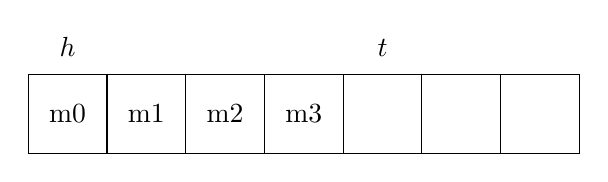
\begin{tikzpicture}

\coordinate (s) at (0,0);
\foreach \num in {0,...,6}{
    \ifthenelse{\num < 4}
    {\node[draw, minimum size=1cm] at (s) (\num) {m\num};} % Fill the box
    {\node[draw, minimum size=1cm] at (s) (\num) {};} % Don't fill the box

    \coordinate (s) at ($(s) + (1,0)$);
}

\node[above=1mm of 0] {$h$};
\node[above=1mm of 4] {$t$};

\end{tikzpicture}

    \caption{Messages are read from the head of the queue ($h$)}
    \label{fig:tikz:queueArrayInitial}
  \end{subfigure}

  \begin{subfigure}[b]{\textwidth}
    \centering
    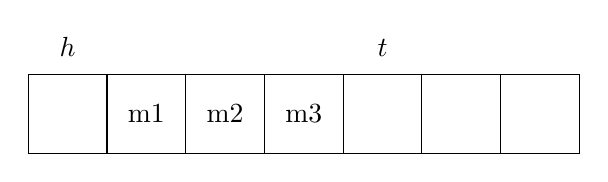
\begin{tikzpicture}

\coordinate (s) at (0,0);
\foreach \num in {0,...,6}{
    \ifthenelse{\num > 0 \AND \num < 4}
    {\node[draw, minimum size=1cm] at (s) (\num) {m\num};} % Fill the box
    {\node[draw, minimum size=1cm] at (s) (\num) {};} % Don't fill the box

    \coordinate (s) at ($(s) + (1,0)$);
}

\node[above=1mm of 0] {$h$};
\node[above=1mm of 4] {$t$};

\end{tikzpicture}

    \caption{The array is shuffled down}
    \label{fig:tikz:queueArrayHeadRead}
  \end{subfigure}

  \begin{subfigure}[b]{\textwidth}
    \centering
    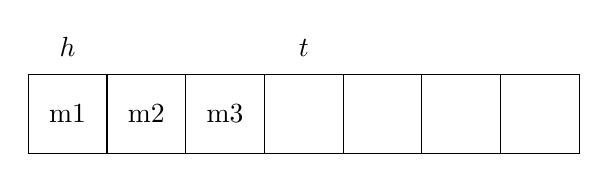
\begin{tikzpicture}

\coordinate (s) at (0,0);
\foreach \num in {1,...,7}{
    \ifthenelse{\num < 4}
    {\node[draw, minimum size=1cm] at (s) (\num) {m\num};} % Fill the box
    {\node[draw, minimum size=1cm] at (s) (\num) {};} % Don't fill the box

    \coordinate (s) at ($(s) + (1,0)$);
}

\node[above=1mm of 1] {$h$};
\node[above=1mm of 4] {$t$};

\end{tikzpicture}

    \caption{The next message is now ready to be read}
    \label{fig:tikz:queueArrayPostShuffle}
  \end{subfigure}
  \caption{Reading a message from an array-based queue}
  \label{fig:tikz:queueArray}
\end{figure}

However, there are several disadvantages of this approach, for both the enqueue and dequeue operations.

\begin{description}
  \item[\textit{enqueue(m)}] \hfill \\
    Arrays in GoLang have a fixed length - but there is no limit on the number
    of messages a queue may be asked to buffer. We can compensate for this by
    using 'slices' instead of arrays\todo{Explain slices - seperate section} -
    which are expandable using the \mintinline{go}{append()} command
    (Listing~\ref{lst:golangAppendToSlice}). The message $m$ is stored into the
    first available array index, which will typically complete in $O(1)$ time.
    However, in order to create the illusion of an 'expandable' array, slices
    use a fixed-length array under the hood - which is expanded when full. This
    expansion involves creating a new array, which is twice the size of the
    original. Each message in the underlying array is then copied to the new
    array, which is used for all slice actions going forward. Therefore, whilst
    the vast majority of messages will be stored in $O(1)$ time, a message that
    triggers an expansion of the underlying array will require $O(n)$ time to
    store (where $n$ is the number of messages in the queue)\todo{Improve
    notation}.
  \item[\textit{dequeue()}] \hfill \\
    Pulling the first message in the array requires that the array be shuffled
    after each \mintinline{go}{dequeue()} operation, so that the next message to
    be delivered always resides in  array position 0 (see in
    Figure~\ref{fig:tikz:queueArray}). An array implementation would be
    extremely inefficient, requiring $n - 1$ items to moved down an array
    position. However, because a slice is simply a 'view' onto an array, this
    operation can be made extremely efficient - by simply creating a new slice,
    with all but the first element in common with the original.\todo{Diagram?}
    It is therefore possible to complete this operation in $O(1)$ time.
\end{description}

\begin{listing}[H]
  \centering
  \inputminted[firstline=7, lastline=12]{go}{code/snippets/appendToSlice.go}
  \caption{An example of appending to a GoLang slice}
  \label{lst:golangAppendToSlice}
\end{listing}

In addition to the disadvantages given above, slices are quite inefficient when
it comes to memory utilisation. At any moment in time, up to 50\% of the
underlying array will be empty. Whilst these array indexes do not contain
messages, they still occupy space in memory, meaning that (in the worst case
scenario) $O(2n)$ space is required to store $n$ messages. This is not ideal.

An alternative method of representing an in-memory-queue, is a linked list
(Figure~\ref{fig:tikz:queueLinkedList}). This has numerous advantages over an
array - with both enqueue and dequeue operations completing in $O(1)$ time.
Linked lists also improve on the space complexity of the queue, as the
datastructure grows and shrinks in response  to the number of messages - meaning
that we require $O(n)$ memory to store $n$ messages.

\begin{description}
  \item[\textit{enqueue(m)}] \hfill \\
    The item at the tail of the queue ($t$) - seen in
    Figure~\ref{fig:tikz:queueLinkedListInitial} - is simply updated with a
    pointer to $m$. This is an $O(1)$ operation, and simple to perform.
  \item[\textit{dequeue()}] \hfill \\
    The item at the head of the queue ($h$) is returned. The head pointer is
    then updated to point to the next message to be read, as in
    Figure~\ref{fig:tikz:queueLinkedListHeadRead}.
\end{description}

\begin{figure}[H]
  \centering
  \begin{subfigure}[b]{\textwidth}
    \centering
    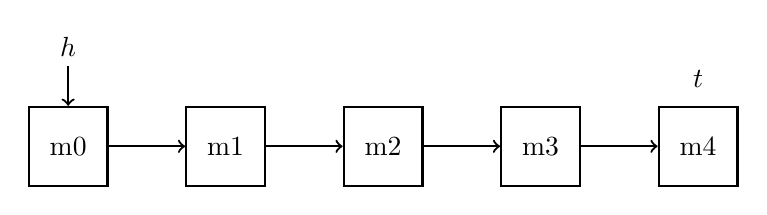
\begin{tikzpicture}[thick]

\coordinate (s) at (0,0);
\foreach \num[remember=\num as \previous] in {0,...,4}{
    \node[draw, minimum size=1cm] at (s) (\num) {m\num};

    \ifthenelse{\num > 0}
    {\draw[->](\previous) edge (\num);}
    {}

    \coordinate (s) at ($(s) + (2,0)$);
}


\node[above=0.5cm of 0] (head) {$h$};
\node[above=1mm of 4] {$t$};
\draw[->,thick](head) edge (0);

\end{tikzpicture}

    \caption{Messages are read from the head of the queue ($h$)}
    \label{fig:tikz:queueLinkedListInitial}
  \end{subfigure}

  \begin{subfigure}[b]{\textwidth}
    \centering
    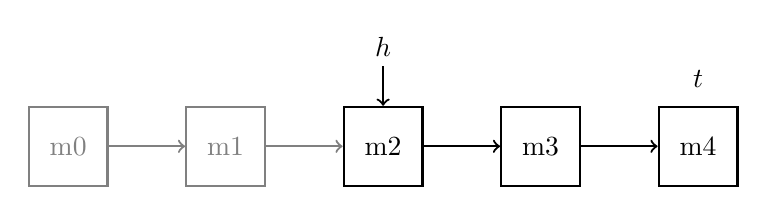
\begin{tikzpicture}[thick]

\coordinate (s) at (0,0);
\foreach \num[remember=\num as \previous] in {0,...,4}{
    \ifthenelse{\num < 2}
    {\node[draw, minimum size=1cm, gray] at (s) (\num) {m\num};}
    {\node[draw, minimum size=1cm] at (s) (\num) {m\num};}

    \ifthenelse{\num < 3}
    {\ifthenelse{\num > 0}{\draw[->, gray](\previous) edge (\num);}{}}
    {\draw[->](\previous) edge (\num);}

    \coordinate (s) at ($(s) + (2,0)$);
}


\node[above=0.5cm of 2] (head) {$h$};
\node[above=1mm of 4] {$t$};
\draw[->](head) edge (2);

\end{tikzpicture}

    \caption{Head moves, and read nodes are marked for garbage collection}
    \label{fig:tikz:queueLinkedListHeadRead}
  \end{subfigure}

  \begin{subfigure}[b]{\textwidth}
    \centering
    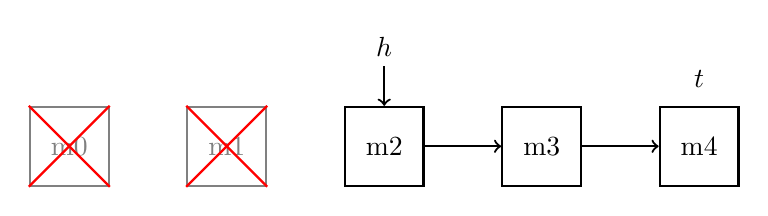
\begin{tikzpicture}[thick]

\coordinate (s) at (0,0);
\foreach \num[remember=\num as \previous] in {0,...,4}{
    \ifthenelse{\num < 2}
    { % These have been garbage collected
      \node[draw, minimum size=1cm, gray] at (s) (\num) {m\num};
      \node(Cross) [draw,cross out,minimum width=1cm,minimum height=1cm,red] at (s) {};
    }
    { % These are still active
      \node[draw, minimum size=1cm] at (s) (\num) {m\num};
    }

    % Don't draw 'next' pointers for dead nodes
    \ifthenelse{\num > 2}{\draw[->](\previous) edge (\num);}{}

    \coordinate (s) at ($(s) + (2,0)$);
}

\node[above=0.5cm of 2] (head) {$h$};
\node[above=1mm of 4] {$t$};
\draw[->](head) edge (2);

\end{tikzpicture}

    \caption{At some point in the future (depending on memory pressure), the
             \gls{gc} will automatically clean up the read messages}
    \label{fig:tikz:queueLinkedListGCRun}
  \end{subfigure}
  \caption{Reading a message from an array-based queue}
  \label{fig:tikz:queueLinkedList}
\end{figure}

A full implementation of a linked list queue can be found in
Appendix~\ref{appendix:queueCode}.

When it comes to representing topics, the situation is similar. As mentioned in
Section~\ref{sub:topics}, the main difference between queues and topics, is the
fact that queues deliver each message to a single consumer, whereas topics
deliver each message to \emph{all} consumers. This requires a subtly different
datastructure to hold the messages - as consumers may read messages at different
rates.\todo{Figure} If we use an array-based datastructure, similar to that in
Figure~\ref{fig:tikz:queueArray}, we would be required to maintain a seperate
queue for each subscriber\todo{Figure} to read from. A topic with $s$
subscribers, and $n$ pending messages would therefore require at \emph{least}
$O(n * s)$ memory, and that is without considering the caveats described
above\todo{XReference}. \\

A linked-list implementation, however, has the potential to be highly efficient
when it comes to storage space. Rather than storing $s$ messages, we can simply
keep multiple 'head' pointers on the same linked-list, one for each subscriber.
When a subscriber consumes a message - only the head pointer belonging to it is
moved up the list, the rest remain static. This method only requires $O(s + m)$
memory, for a topic with $s$ subscribers, and $m$ messages. The linked-list
implementation of a topic therefore has an even bigger efficiency saving over
the corresponding array-based implementation, than in the queue examples given
above, as seen in Figure~\ref{fig:tikz:implementationSpaceComplexityGraph}.

\begin{figure}[H]
  \centering
  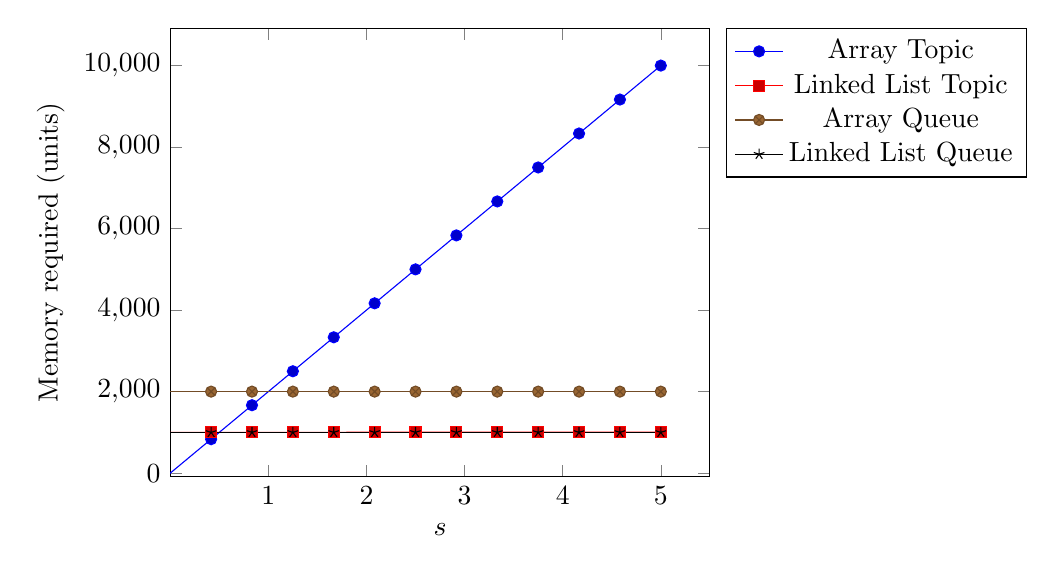
\begin{tikzpicture}
\begin{axis}[
    xlabel=$s$,
    ylabel={Memory required (units)},
    xmin=0,
    xtick={1,...,10},
    scaled ticks=false,
    legend entries={Array Topic, Linked List Topic, Array Queue, Linked List Queue},
    legend pos=outer north east,
]
\addplot {2 * x * 1000};
\addplot {x + 1000};
\addplot {2 * 1000};
\addplot {1000};
\end{axis}
\end{tikzpicture}

  \caption{A comparison of the space complexities of various queue/topic
           implementations, as the number of subscribers ($s$) increases}
  \label{fig:tikz:implementationSpaceComplexityGraph}
\end{figure}

\subsection{Message Shipper}
\label{sub:Message Shipper}

\todo[inline]{Message delivery/queue/topic behavior}

\subsection{Metrics Manager}
\label{sub:Metrics Manager}

\todo[inline]{Metric format/serialization. How do we ensure minimal CPU usage}

\section{Presentation Interface}
\label{sec:Presentation Interface}

\todo[inline]{Screenshots/high-level description}

\subsection{Graphite/Grafana}
\label{sub:Graphite/Grafana}

\todo[inline]{Architecture}

\subsection{Docker}
\label{sub:Docker}

\todo[inline]{Overview and Dockerfile description}

\section{Utilities}
\label{sec:Utilities}

\todo[inline]{Python benchmark code walkthrough}

\subsection{Configuration}
\label{sub:Configuration}

\todo[inline]{Specifics of command-line flag/config file implementation}


  \chapter{Testing and Evaluation}
\label{chap:Testing and Evaluation}

\section{Unit Tests}
\label{sec:Unit Tests}

\todo[inline]{GoLang unit test structure.}

\subsection{Asynchronous Testing}
\label{sub:Asynchronous Testing}

\todo[inline]{Difficulties associated with async testing/Gomega etc.}

\subsection{TravisCI}
\label{sub:TravisCI}

\missingfigure{Travis.CI screenshot}

Despite my initial plan being to set up and host most of my Continuous
Integration infrastructure myself, it became clear after an initial trial that
it would be far easier for me to ensure build repeatability/speed if I used a
cloud-based CI service (some of the reasons for which are detailed below). With
this in mind, I elected to use the popular and excellent
\href{https://travis-ci.org/}{Travis CI} - which provides a free tier for
open-source projects such as mine. Setup was as simple as adding a `.travis.yml`
file to my project, and enabling my GitHub repo for builds on the Travis CI
admin panel. My initial .travis.yml file can be seen in
Listing~\ref{lst:initialTravis}, and the latest version is available
\href{https://github.com/FireEater64/gamq/blob/master/.travis.yml}{on GitHub}.
There are a multitude of configurable options available\footnote{More
information on the contents of .travis.yml files can be found in their
\href{https://docs.travis-ci.com/}{excellent documentation}.}, but my initial
configuration in Listing~\ref{lst:initialTravis} consisted of only three:

\begin{listing}
  \centering
  \begin{minted}[frame=single,framesep=10pt]{YAML}
language: go

go:
  - 1.3
  - 1.4
  - tip

script: go test -v ./... -bench=.
  \end{minted}
  \caption{Initial .travis.yml}
  \label{lst:initialTravis}
\end{listing}

\begin{description}
  \item[Language] Defines the language of the project being built - in this case
  \href{https://golang.org/}{GoLang}. TravisCI builds (usually) take place
  inside \href{https://www.docker.com/what-docker}{Docker containers}, with the
  'language' section of configuration dictating which pre-built container is
  used for this particular build. In this case, a language value of 'go' will
  ensure that the build container contains all of the binaries and environment
  variables required for building and running GoLang projects.
  \item[Go] This section defines different versions of the go compiler you wish
  to build your product on. When code is checked in - Travis will spin up a
  separate container for each version specified, and run your complete test
  suite inside each container in parallel. This feature is known as the
  '\href{https://docs.travis-ci.com/user/customizing-the-build/#Build-Matrix}{build
  matrix}', and is both \emph{incredibly} useful for ensuring software
  consistency on multiple different compilers/runtimes (especially useful for
  interpreted languages such as Java), and something which would be hard to
  replicate outside of a containerised build environment (i.e. if I'd chosen to
  self-host my CI).
  \item[Script] Any custom commands you wish to be run as part of the build.
  Travis contains (pun intended) a standard build script for most languages
  (which are selected via the 'language' configuration detailed above), however
  builds invariably require additional scripts/commands to be run as well - some
  example use cases could be to run additional tests, or deploy build binaries
  to an artifact repository. In this case, the commands I specified execute both
  my unit/integration test suite, and my benchmark suite (more details below).
\end{description}

\subsection{Coveralls}
\label{sub:Coveralls}

\missingfigure{Coveralls screenshot}

One important (though not definitive) metric associated with unit/integration
tests is \emph{code coverage}, which is the total percentage of the code-base
that is executed when running unit tests. This is a useful metric to keep an eye
on, as it helps\footnote{Though doesn't always} indicate which sections of code
are susceptible to bugs as a result of not being tested. Go's built in test
runner is capable of producing code coverage reports during test runs, however I
chose to use an open source tool called
'\href{https://github.com/axw/gocov}{gocov}', as it allowed me to send the code
quality metrics produced my build to another online service,
\href{https://coveralls.io/}{coveralls}. The reasons behind doing this, rather
than relying on the build-in HTML report were:

\begin{description}
  \item[Visibility] Publishing my code quality metrics in an easily accessibly,
  publicly visible website (as well as the front page of my GitHub project),
  rather than hiding them away in build logs helps to 'keep me honest', as well
  as '\textit{\gls{gamify}}' the process of driving up coverage.
  \item[Monitoring] Coveralls allows me to set 'thresholds' for coverage
  metrics, and will fail the build if these are not adhered to. For example, my
  build will fail if the coverage of the checked in code is even 0.1\% less than
  that of the previous successful build.
\end{description}

The code quality metrics for my project are available
\href{https://coveralls.io/github/FireEater64/gamq?branch=master}{on Coveralls},
as well as being summarised in the
\href{https://github.com/FireEater64/gamq/blob/master/README.md}{README for my
project on GitHub}\(Figure~\ref{fig:readmeStatus} \).

\begin{figure}
  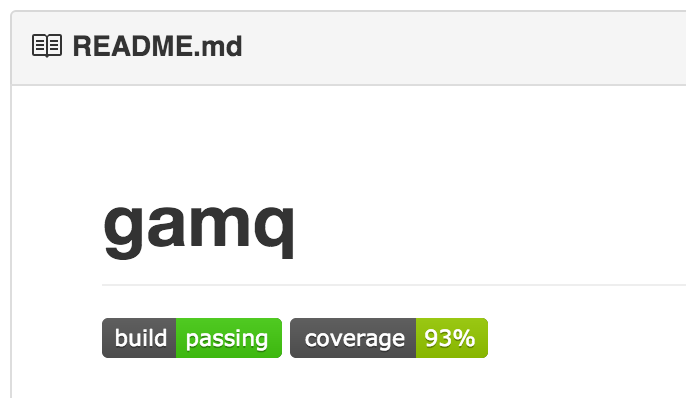
\includegraphics{figures/README}
  \centering
  \caption{Code status badges in README.md}
  \label{fig:readmeStatus}
\end{figure}

\section{Environmental Testing}
\label{sec:Environmental Testing}

\todo[inline]{Importance of \emph{doing} environmental testing}

\subsection{Methodology}
\label{sub:Methodology}

\todo[inline]{Prof files/timings etc.}

\subsection{Tools}
\label{sub:Tools}

\todo[inline]{Network link conditioner/test scripts/presentation framework}

\section{System Performance}
\label{sec:System Performance}

\todo[inline]{Analysis of prof files/theoretical maximum limits/comparisons/potential improvements}


  \chapter{Conclusion}
\label{chap:Conclusion}

Overall, the project was an excellent learning experience. It provided an
opportunity to learn a new programming language and explore modern, open-source
development techniques - as well as learn about the intricacies involved with
building infrastructure software, the complexities of which are often
overlooked.

\section{Project Goals}
\label{sec:goalsConclusion}

The goal of this project has changed multiple times over the last 8 months.
Initial plans, were to build a very simple message broker - to be used as a
vehicle for exploring autonomic computing principals, and create a
'self-healing', 'self-improving' message broker. These goals were made with no
knowledge of the challenges associated with learning a new language like Go, and
in dealing with the complexities of parallelism at the scale used in \gls{gamq}.
During a mid-project review it was decided that, whilst it was theoretically
possible that the complexity of the broker could be scaled down, and the
original project goals still met - the goal of the project should be refocused
towards producing a mature, high-performance, well-tested messaging broker. This
reflected not only the reality of the situation at the time, but a change in the
authors interests. These new goals, the ones outlined in
Chapter~\ref{chap:Introduction} have, as far as the author is concerned, all
been met - and the decision to change the project focus was, in hindsight, the
correct one.

\subsection{Experience with GoLang}
\label{sub:golangConclusion}

After completing the authors first substantial piece of work with the Go
programming language, the power of CSP-style concurrency, combined with a clean,
modern development infrastructure - demonstrate why Go is now one of the top 20
most popular languages on GitHub\cite{languageRankings}, despite its young age.
Whilst it is arguable that a broker with similar feature-set could have been
produced in a more familiar language\footnote{Such as Python, or Java} in less
time, the performance and scalability of the implementation would have almost
certainly lagged behind that of gamq.

\subsection{Performance}
\label{sub:performance}

Whilst the performance of gamq (Section~\ref{sec:systemPerformance}) is
considerably higher than originally hoped (original estimates predicted
somewhere in the region of 5,000 messages/second), there are still numerous
potential performance increases that could be explored. The biggest of these
(according to the CPU performance profile in
Appendix~\ref{appendix:profileResults}) lies in reducing the amount of garbage
created by the application (and consequently, the amount of time spent
performing garbage collection), through the reuse of message objects, and the
use of zero-allocation buffers \cite{highPerformanceSystemsInGo} when receiving
data.

\section{Future Work}
\label{sec:Future Work}

Going forward, it is hoped that some of the knowledge (and possibly code!) gained
from this project continue to see use in some form or another. Towards the end
of the project, the 'professional open-source' message broker
NATS\footnote{\url{https://nats.io/}} was examined for similarities/differences
with gamq. Whilst the size and scope of NATS far outstrips that of gamq, it is
hoped that it will be possible to transfer some of the knowledge gained during
this project in the form of open-source
contributions\footnote{\url{https://github.com/nats-io/gnatsd/pulls}}
to other projects like NATS.


  \begin{appendix}
    \chapter{Project Gantt Chart}
\label{appendix:ganttChart}

\begin{ganttchart}[
  hgrid,
  vgrid,
  today=23,
  today rule/.style=%
    {draw=blue, ultra thick}
  ]{1}{23}

  % Titles
  \gantttitle{Semester 1}{12}
  \gantttitle{Semester 2}{11} \\
  \gantttitlelist{1,...,12}{1}
  \gantttitlelist{1,...,11}{1} \\

  % Groups
  \ganttgroup{Seminar}{8}{8} \\
  \ganttgroup{Presentation of results}{18}{20} \\

  % Deadlines
  \ganttmilestone{Code freeze/submission}{19} \\
  \ganttmilestone{Project showcase}{21} \\
  \ganttmilestone{Final report deadline}{23} \\

  % Bars
  \ganttbar{Project plan}{1}{1} \\
  \ganttbar{Research}{2}{6} \\
  \ganttbar{Language Learning}{4}{6} \\
  \ganttbar{Seminar prep}{5}{7} \\
  \ganttbar{First code sprint}{7}{11} \\
  \ganttbar{First retrospective}{12}{12} \\
  \ganttbar{Second code sprint}{13}{17} \\
  \ganttbar{Presentation preparation}{15}{17} \\
  \ganttbar{Bug bash/second retrospective}{18}{19} \\

  \ganttbar{Video creation}{20}{23} \\
  \ganttbar{Report writing}{2}{23}

\end{ganttchart}

\chapter{Queue Code}
\label{appendix:queueCode}

\inputminted[breaklines=true, breakanywhere]{go}{code/gamq/queue/queue.go}

\chapter{UdpWriter}
\label{appendix:udpWriter}

\inputminted[breaklines=true, breakanywhere]{go}{code/gamq/udp/udpwriter.go}

\chapter{Parse Client Command}
\label{appendix:parseClientCommand}

\inputminted[breaklines=true, breakanywhere, firstline=226, lastline=260]{go}{code/gamq/connectionmanager.go}

\chapter{Send Messages To Client}
\label{appendix:sendMessagesToClient}

\inputminted[breaklines=true, breakanywhere, firstline=35, lastline=67]{go}{code/gamq/messageshipper.go}

\chapter{Benchmark Code}
\label{chap:benchmarkCode}

\inputminted[breaklines]{python}{code/gamq/tools/benchmark/benchmark.py}

\chapter{Test Output}
\label{chap:testOutput}

\inputminted[breaklines]{bash}{code/goTestOutput}

  \end{appendix}

  \newpage

  \printglossaries

  \newpage

  \printbibliography

\end{document}
